\documentclass[journal,onecolumn]{IEEEtran}


\ifCLASSINFOpdf

\else

\fi

\usepackage{tikz}
\usetikzlibrary{shapes.geometric, arrows.meta, positioning}
\usepackage{float}
\usepackage{hyperref}
\usepackage{booktabs}   % Tablas profesionales IEEE
\usepackage{graphicx}   % Inserción de figuras

\hyphenation{op-tical net-works semi-conduc-tor}


\begin{document}

\title{Plataforma de seguridad predictiva para la minería subterránea}


\author{Jazmin Dajerly Moreno Galindo, Sebastian David Lizarazo Duarte\\
Universidad Pedagógica y Tecnológica de Colombia \\
Sogamoso, Colombia \\
jazmin.moreno01@uptc.edu.co\\
sebastian.lizarazo03@uptc.edu.co}


\maketitle

\begin{abstract}


\end{abstract}

\begin{IEEEkeywords}

\end{IEEEkeywords}

\IEEEpeerreviewmaketitle



\section{Introduction}
La minería subterránea de carbón figura entre las actividades con mayor índice de accidentalidad en el mundo. Según estimaciones de la Organización Internacional del Trabajo (OIT), por cada minero que muere en una mina, al menos diez quedan con lesiones permanentes \cite{oms}. En Colombia esta situación es especialmente preocupante puesto que el sector minero supera los índices de accidentalidad de otras industrias, y los incidentes asociados a gases tóxicos, falta de oxígeno y explosiones de metano encabezan las causas de muerte entre los trabajadores \cite{decreto1886}. Por esto, tener sistemas capaces de monitorear las condiciones del ambiente subterráneo y anticipar eventos peligrosos es una necesidad real.
Los sistemas de monitoreo que se usan hoy en la mayoría de las minas funcionan comparando las lecturas de los sensores contra umbrales fijos establecidos por la normativa. El problema es que solo generan una alerta cuando el límite ya se superó, lo que deja poco margen de reacción, sobre todo en situaciones que se desarrollan rápidamente. La atmósfera dentro de una mina cambia constantemente por factores como la ventilación, las voladuras, los equipos diésel y la propia geología del terreno. Frente a esa variabilidad, un sistema útil no debería limitarse a reportar lo que ya pasó, sino anticipar lo que puede pasar con el tiempo suficiente para evacuar si es necesario.
En los últimos años, el aprendizaje automático ha dado herramientas concretas para atacar este problema. Las redes LSTM (Long Short-Term Memory) han mostrado buenos resultados modelando series temporales de gases porque capturan dependencias a lo largo del tiempo \cite{hochreiter1997}. Por su parte, Isolation Forest permite detectar anomalías en datos multivariados, lo que lo hace más potente que los controles tradicionales que analizan cada variable por separado \cite{liu2008}. A esto se suma que los modelos de lenguaje de gran escala (LLM) combinados con sistemas de recuperación de información (RAG) abren la posibilidad de consultar normativa técnica de forma automática y generar diagnósticos en lenguaje natural comprensible para los operadores \cite{lewis2020, gemini}.
El inconveniente es que la mayoría de los trabajos proponen estas soluciones por separado: el modelo predictivo por un lado, el sistema de alertas por otro, y la consulta normativa de forma manual. Esa fragmentación impide tener una visión integrada del riesgo, donde todas las piezas funcionen juntas.
\subsection{Contribución}
Este artículo propone una plataforma de seguridad predictiva para minería subterránea construida sobre una arquitectura multiagente orquestada con LangGraph. El sistema integra cuatro componentes: (i) un modelo LSTM que predice la evolución de gases con un horizonte de 90 minutos, (ii) un detector Isolation Forest para anomalías multivariadas, (iii) un motor RAG que consulta semánticamente el corpus normativo colombiano, y (iv) el LLM Gemini 1.5 Flash para generar diagnósticos con contexto. Estos componentes se coordinan a través de un grafo de ejecución cíclico que mantiene estado entre ciclos, lo que le da al sistema memoria acumulativa por zona minera.
Frente a otros trabajos del área, esta propuesta se distingue en tres puntos: primero, combinar predicción temporal y detección de anomalías en un mismo agente crea dos capas de defensa que se complementan; segundo, el uso de RAG junto con un LLM permite que el sistema no solo identifique el riesgo, sino que justifique su diagnóstico con base en la normativa vigente; tercero, la orquestación con LangGraph hace que agregar nuevos agentes, como uno para análisis geomecánico, uno de visión por imágenes, no requiera modificar los ya existentes.
\subsection{Estructura del artículo}
El resto del documento se organiza así: la Sección~\ref{sec:related_work} revisa los antecedentes en monitoreo inteligente de minas y uso de aprendizaje automático en seguridad minera. La Sección~\ref{sec:materials} detalla la arquitectura, los modelos y el flujo de orquestación. La Sección~\ref{sec:results} presenta y discute los resultados experimentales. Por último, las Secciones~\ref{sec:conclusions} y~\ref{sec:future_work} recogen las conclusiones y las líneas de trabajo futuro.

\section{Related Work}
\label{sec:related_work}
La literatura reciente en seguridad minera ha explorado el uso de agentes especializados que trabajan en paralelo sobre distintas variables del entorno subterráneo. Cai et al. \cite{cai2021} trabajaron en esa dirección: su sistema combina análisis de gases, predicción temporal y detección de anomalías bajo un esquema cooperativo aplicado a minas de carbón. El planteamiento es similar al de este artículo en varios puntos, sin embargo, su arquitectura no incluye modelos de lenguaje ni mecanismos para consultar normativa de forma automática. Esa brecha es justamente lo que motiva parte del diseño propuesto aquí.

El problema de detectar anomalías cuando intervienen múltiples variables al mismo tiempo tiene sus propias complejidades. Un sensor puede estar dentro del rango permitido y aun así formar parte de una condición peligrosa si otros sensores también muestran desviaciones menores de forma simultánea. Para este tipo de situaciones, Liu et al. \cite{liu2008} propusieron Isolation Forest, un algoritmo que aprovecha la facilidad con la que los datos atípicos se separan del resto al construir árboles de decisión aleatorios. En la práctica industrial ha demostrado ventajas claras frente a los controles univariados, precisamente porque captura esas interacciones entre variables que los umbrales individuales no alcanzan a cubrir.

\section{Materials and Methods}
\label{sec:materials}
\subsection{Zonas de Estudio y Datos de Sensores}
El sistema fue diseñado para monitorear cuatro zonas estratégicas de una mina subterránea de carbón simulada en el departamento de Boyacá, Colombia: \textit{Frente\_A\_Sogamoso}, \textit{Frente\_B\_Mongua}, \textit{Galeria\_Central} y \textit{Bocamina}. Se monitorean una serie de gases que incluyen metano (CH$_4$), monóxido de carbono (CO), dióxido de carbono (CO$_2$), oxígeno (O$_2$) y sulfuro de hidrógeno (H$_2$S), además de temperatura y humedad relativa. Los datos se generaron por un simulador calibrado según el Decreto 1886/2015 (Arts. 39, 40, 44) \cite{decreto1886}, con tres niveles de comportamiento de los gases: normal (80\% de los ciclos), perturbación (15\%) e incidente (5\%). Esta distribución refleja la realidad de una mina subterránea, donde la mayoría de los ciclos corresponden a condiciones normales, con la presencia esporádica de eventos menores y donde los incidentes de seguridad reales son escasos. Este conjunto de datos sintéticos fue utilizado para el desarrollo y validación del sistema, dado que los modelos LSTM fueron entrenados con datos representativos de operaciones mineras reales y el simulador reproduce los rangos normativos internacionales (NIOSH \cite{nioshidlh}, OSHA \cite{osha146}) y nacionales.

\subsection{Arquitectura Multiagente}
El sistema emplea una arquitectura multiagente basada en el patrón Orquestador-Especialista \cite{wooldridge1995}; el diagrama de la arquitectura se presenta en la Figure \ref{fig:system_architecture}.

\begin{figure}[H]
    \centering
    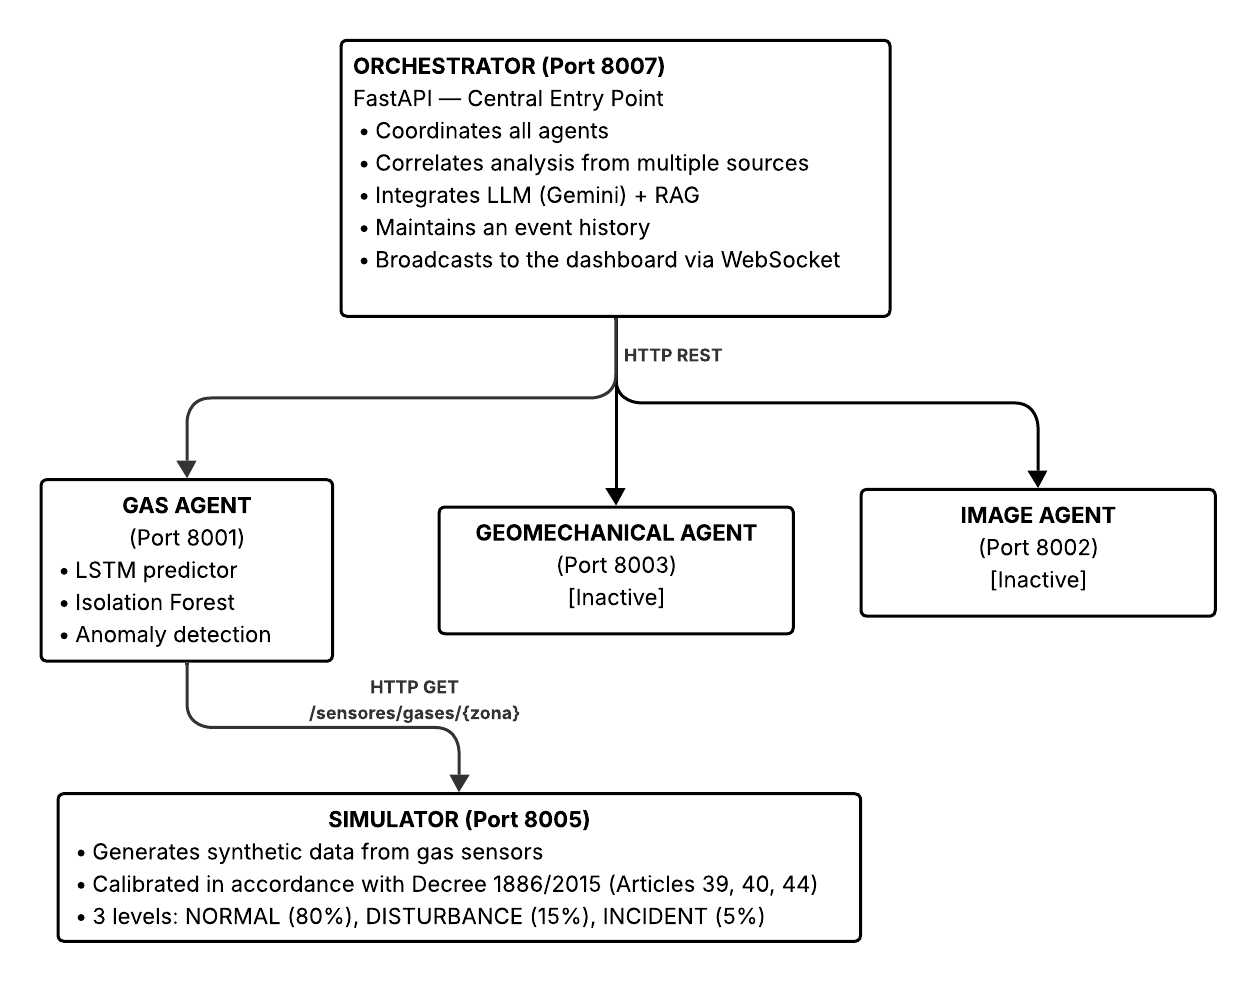
\includegraphics[width=0.7\textwidth]{images/system-architecture.png}
    \caption{Arquitectura del sistema multiagente}
    \label{fig:system_architecture}
\end {figure}

\begin{itemize}
    \item \textbf{Orquestador (Puerto 8007):} Es el punto de entrada central implementado con FastAPI. Se encarga de coordinar todos los agentes, conecta el análisis de múltiples fuentes, integra el motor LLM y RAG, y transmite eventos al dashboard mediante WebSocket.
    \item \textbf{Agente de Gases (Puerto 8001):} Analiza lecturas de sensores simulados teniendo en cuenta los umbrales normativos, predice anomalías utilizando Long Short-Term Memory (LSTM) y las detecta mediante Isolation Forest. Finalmente, mantiene un historial de 500 lecturas por zona en SQLite.
    \item \textbf{Simulador (Puerto 8005):} Genera datos sintéticos de los sensores simulados calibrados según rangos internacionales (NIOSH, OSHA) y nacionales (Decreto 1886/2015).
\end{itemize}

\subsection{Clasificación de Riesgo por Umbrales Normativos}
La clasificación de riesgo se basa en los niveles establecidos por el Decreto 1886 de 2015 (Art. 39, 40, 118, 120, 123) \cite{decreto1886}. Dichos niveles son presentados en la Table \ref{tab:umbrales}.

\begin{table}[H]
\centering
\caption{Umbrales de clasificación de riesgo por gas (Decreto 1886/2015)}
\label{tab:umbrales}
\begin{tabular}{l|c|c|c|c}
\toprule
\textbf{Gas} & \textbf{SEGURO} & \textbf{PRECAUCIÓN} & \textbf{RIESGO ALTO} & \textbf{EVACUACIÓN} \\
\midrule
CH$_4$ (\% vol.) & $<$1.0 & 1.0--1.49 & 1.5--4.99 & $\geq$5.0 \\
CO (ppm) & $<$25 & 25--49.9 & 50--199.9 & $\geq$200 \\
CO$_2$ (\% vol.) & $<$0.5 & 0.5--2.99 & 3.0--4.99 & $\geq$5.0 \\
O$_2$ (\% vol.) & 19.5--23.5 & 17.5--19.49 & 16.0--17.49 & $<$16.0 \\
H$_2$S (ppm) & $<$1.0 & 1.0--4.9 & 5.0--49.9 & $\geq$50 \\
\bottomrule
\end{tabular}
\end{table}

\subsection{Modelo LSTM para Predicción de Series Temporales}
Para predecir la evolución de los niveles de gases en un horizonte de 90 minutos, se implementó un modelo LSTM (\textit{Long Short-Term Memory}) basado en la arquitectura propuesta por Hochreiter y Schmidhuber \cite{hochreiter1997}. Este modelo posee una capacidad de aprender dependencias temporales de largo plazo en secuencias donde intervienen múltiples variables, situación presente en la dinámica de gases subterráneos, donde un evento adverso puede tener precursoras varias horas antes de manifestarse.

\subsubsection{Arquitectura del modelo}
El modelo recibe como entrada una ventana histórica de 24 lecturas de gases (correspondientes a 6 horas de monitoreo, con una lectura cada 15 minutos). Cada lectura contiene cinco variables: CH$_4$, CO, O$_2$, CO$_2$ y H$_2$S, por lo que la forma de entrada es $(24, 5)$. La arquitectura está compuesta por dos capas LSTM apiladas:\\

\begin{itemize}
    \item \textbf{Capa LSTM 1:} 128 unidades con \texttt{return\_sequences=True}. Esta configuración permite que la capa devuelva la salida en cada paso temporal, alimentando así a la segunda capa.
    \item \textbf{Capa LSTM 2:} 64 unidades con \texttt{return\_sequences=False}. Procesa la secuencia completa y devuelve únicamente el último vector de estado, capturando la representación resumida de toda la ventana histórica.
    \item \textbf{Capa de salida:} Dense(30) seguida de un \texttt{reshape} a $(6, 5)$. Los 30 valores se reorganizan en 6 pasos temporales (90 minutos de predicción) $\times$ 5 gases.
\end{itemize}
La Figure \ref{fig:lstm_architecture} ilustra el flujo de datos a través de las capas.

\begin{figure}[H]
 \centering
    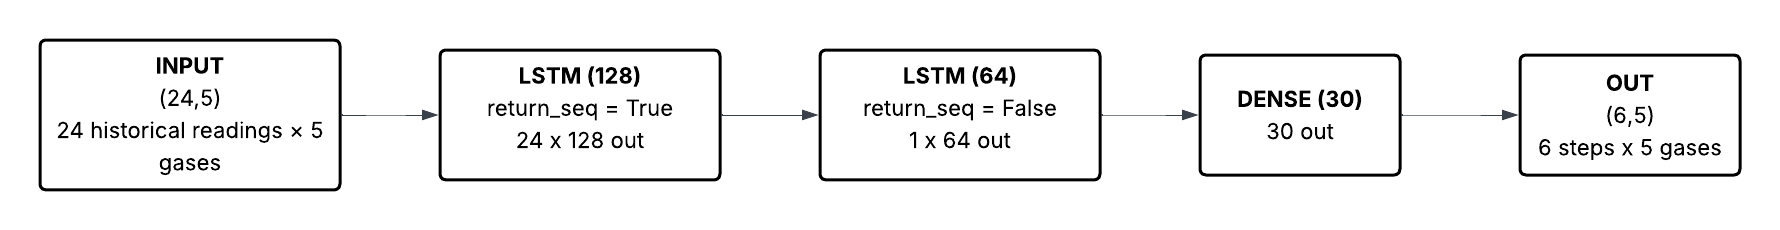
\includegraphics[width=1\textwidth]{images/lstm-architecture.png}
    \caption{Arquitectura del modelo LSTM.}
    \label{fig:lstm_architecture}
\end{figure}

\subsubsection{Entrenamiento}
Cada modelo se entrenó utilizando Keras 3.13.2 \cite{keras} en Google Colab, el cual es un entorno de Jupyter notebook en la nube con acceso a GPUs NVIDIA Tesla T4. A cada zona de monitoreo se le efectuó un entrenamiento independiente, generando así cuatro modelos:

\begin{itemize}
    \item LSTM zona Bocamina
    \item LSTM zona Frente A (Sogamoso)
    \item LSTM zona Frente B (Mongua)
    \item LSTM zona Galería Central
\end{itemize}

Una vez finalizado el entrenamiento, cada modelo se almacenó en formato \texttt{.keras}. Este formato empaqueta a manera de ZIP la arquitectura de la red, los pesos que se aprendieron durante el entrenamiento y la configuración del optimizador. Su carga y despliegue resultan sencillos gracias a su compresión.\\

\subsubsection{Inferencia en producción}
Se estableció a manera de diseño arquitectónico que el sistema \textbf{no utilice TensorFlow ni Keras en runtime}. La inferencia se realiza en \textbf{NumPy puro} mediante la lectura directa de los pesos H5 con la biblioteca \texttt{h5py}. Este enfoque se implementó dada la ausencia de GPUs en los computadores de prueba, y la necesidad de minimizar las dependencias runtime para facilitar el despliegue en entornos controlados. Los pesos se cargan directamente desde el archivo H5 contenido en el \texttt{.keras} y se aplica la propagación hacia adelante (\textit{forward-pass}) utilizando únicamente las operaciones de álgebra lineal de NumPy. Esta estrategia reduce de manera significativa el consumo de memoria y permite que el sistema se pueda operar en servidores sin aceleración por hardware, manteniendo la capacidad predictiva del modelo entrenado.

\subsection{Detección de Anomalías con Isolation Forest}
Para complementar al LSTM, se empleó un modelo basado en árboles de decisión llamado \textit{Isolation Forest} \cite{liu2008} el cual se encarga de detectar anomalías en las variables que se están evaluando. Mientras LSTM predice la evolución de los gases a través del tiempo, \textit{Isolation Forest} identifica patrones que se alejan del comportamiento normal. 

El modelo opera sobre cinco características que capturan las relaciones entre las variables que no son identificables cuando se analiza cada gas de forma aislada:

\begin{enumerate}
    \item \textbf{Ratio CH$_4$/CO:} A partir del calculo de CH$_4$ / (CO + $\varepsilon$) un resultado elevado indica actividad de combustión lo que puede revelar un incendio incipiente antes de que los umbrales individuales se activen.
    \item \textbf{Déficit de O$_2$:} Con $\max(0, 20.5 - O_2)$ se puede calcular cuánto falta para alcanzar el nivel mínimo aceptable de oxígeno.
    \item \textbf{Gas composite score:} $\sum_i (valor_i / umbral_i)$. Puntuación de peligrosidad multigas, donde cada gas se pondera por su umbral de alarma según el Artículo 39 del Decreto 1886/2015~\cite{decreto1886}.
    \item \textbf{$\Delta$CH$_4$:} Variación de metano en el último intervalo (CH$_4$(t) $-$ CH$_4$(t$-$1)). Detecta cambios abruptos incluso dentro de rangos que aparentan ser seguros.
    \item \textbf{Índice de estrés térmico:} $T \times (H/100)$. Combina temperatura y humedad relativa para estimar estrés ambiental en galerías profundas.
\end{enumerate}

El modelo también incorpora reglas de detección por incrementos bruscos ($\Delta$ $>$ 50\% para CH$_4$), patrón de incendio (CO y CO$_2$ ascendiendo simultáneamente) y zona de explosividad (CH$_4$ entre 1\% y 5\% vol. con O$_2$ $>$ 12\%).

\subsection{Motor RAG -- Consulta Normativa Semántica}
Se implementó un motor RAG (\textit{Retrieval-Augmented Generation})~\cite{lewis2020} para consultar el corpus normativo colombiano. Este sistema permite que durante una emergencia, el operador le pueda hacer preguntas al sistema y obtenga la respuesta correcta con referencia normativa precisa, sin necesidad de consultar la documentación de manera manual.

\subsubsection{Corpus normativo}
El corpus está contenido en \texttt{corpus\_normativo.json} e incluye:
\begin{itemize}
    \item \textbf{Decreto 1886/2015:} Contiene 140 artículos sobre seguridad minera subterránea en los que se incluye límites de gases, ventilación, planes de emergencia, etc.
    \item \textbf{Estándares internacionales:} OSHA~\cite{osha146}, MSHA~\cite{msha57}, NIOSH IDLH~\cite{nioshidlh}, ACGIH TLV~\cite{acghtlv}.
\end{itemize}

Los artículos están categorizados por gas y tipo de contenido (CH$_4$, CO, CO$_2$, O$_2$, H$_2$S, emergencia), esto con el objetivo de permitir consultas categorizadas.

\subsubsection{Arquitectura del motor}
El motor RAG contiene los siguientes elementos:
\begin{itemize}
    \item \textbf{Embeddings:} Se utiliza el modelo \texttt{all-MiniLM-L6-v2} de HuggingFace que  es capaz de transformar texto en vectores densos de 384 dimensiones. Posee un equilibrio entre velocidad y calidad de representación.
     \item \textbf{Índice vectorial:} FAISS \cite{johnson2019}. Este componente almacena las representaciones vectoriales de los fragmentos normativos y permite recuperar los más relevantes mediante búsquedas por similitud coseno. 
    \item \textbf{Chunking:} LangChain con \texttt{RecursiveCharacterTextSplitter} (chunk size=500, overlap=60). Esta estrategia divide los artículos extensos en fragmentos de menor tamaño, manteniendo la continuidad del contexto entre ellos. De esta forma, cada fragmento puede ser procesado adecuadamente durante la generación de embeddings.
\end{itemize}

\subsubsection{Modos de consulta}

El motor de búsqueda implementado permite realizar consultas normativas de diferentes maneras, dependiendo de las necesidades del usuario:

\begin{itemize}
    \item \textbf{Por texto libre:} \texttt{consultar(query, k=3)}. Este modo recibe una consulta en lenguaje natural y devuelve los \texttt{k} fragmentos normativos con mayor relevancia semántica.
    \item \textbf{Por categoría:} \texttt{consultar(query, k=3, categoria="CH4")}. Además de la consulta en lenguaje natural, permite restringir la búsqueda a una categoría normativa específica, lo que facilita la recuperación de información relacionada con un tema determinado.
\end{itemize}

Para generar respuestas en lenguaje natural, se implementó la función \texttt{consultar\_con\_llm()}. Su funcionamiento consiste en recuperar primero los fragmentos más relevantes mediante FAISS y, posteriormente, proporcionar dicho contexto al modelo Gemini 1.5 Flash. Con esta información, el modelo genera una respuesta fundamentada en el contenido normativo recuperado.

\subsection{Motor LLM -- Razonamiento Contextual}

Para complementar el análisis realizado por los agentes, el sistema incorpora Google Gemini 1.5 Flash \cite{gemini} como modelo de lenguaje encargado de generar diagnósticos y recomendaciones en lenguaje natural. La información suministrada al modelo incluye:

\begin{itemize}
    \item Las lecturas actuales de los gases y su comportamiento reciente.
    \item Los fragmentos normativos recuperados mediante el mecanismo RAG.
    \item Las correlaciones identificadas entre los diferentes agentes del sistema.
    \item El nivel de riesgo global calculado para la mina.
\end{itemize}

Con base en esta información, se construye una instrucción que orienta al modelo para producir un diagnóstico técnico de la situación observada. Además, se solicita la generación de acciones inmediatas priorizadas, la referencia a la normativa aplicable del Decreto 1886 de 2015 y una estimación del comportamiento esperado durante los siguientes 30 minutos.

Como mecanismo de contingencia, el sistema puede operar sin depender del servicio externo del modelo de lenguaje. Cuando la API no se encuentra disponible, ya sea por ausencia de configuración o por restricciones de uso, se emplea un procedimiento alternativo basado en reglas y plantillas predefinidas. En este modo, las concentraciones de gases se evalúan de acuerdo con los umbrales establecidos por la normativa y se generan recomendaciones acordes con el nivel de riesgo detectado.

\subsection{Flujo de Orquestación con LangGraph}
La coordinación de los componentes del sistema se realiza mediante un grafo de ejecución implementado con LangGraph \cite{langgraph}, en el cual se organizar el procesamiento de la información en etapas sucesivas, donde cada nodo aporta información que es utilizada por los nodos posteriores. La representación de este flujo se observa en la Figure \ref{fig:langgraph_flow}.

\begin{figure}[H]
\centering
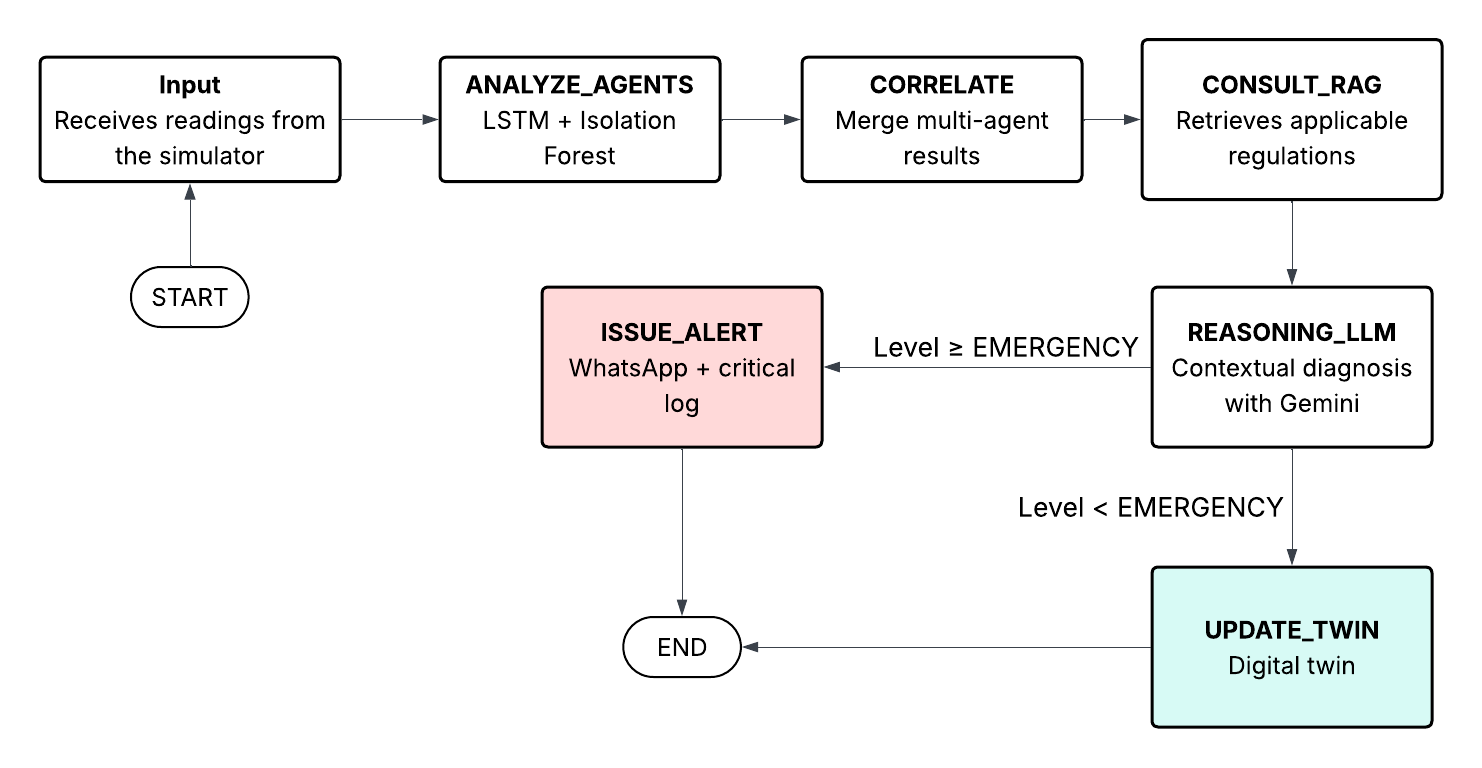
\includegraphics[width=1\textwidth]{images/langgraph-flow.png}
\caption{Grafo de orquestación LangGraph.}
\label{fig:langgraph_flow}
\end{figure}

Los nodos presentes en la Figure \ref{fig:langgraph_flow} poseen responsabilidades especificas que se describen a continuación:
\begin{enumerate}
    \item \textbf{Ingesta:} incorpora las lecturas generadas por el simulador y las almacena en el estado compartido utilizado por el grafo.
    \item \textbf{Analizar agentes:} consulta el Agente de Gases para evaluar las condiciones actuales de la mina. En esta etapa se ejecutan los modelos LSTM para predicción temporal y el algoritmo Isolation Forest para la detección de anomalías.
    \item \textbf{Correlacionar:} integra los resultados obtenidos por los diferentes agentes con el fin de construir una visión consolidada del estado de cada zona minera.
    \item \textbf{Consultar RAG:} identifica y recupera los fragmentos normativos que pueden resultar relevantes para las condiciones detectadas durante el análisis.
    \item \textbf{Razonar LLM:} utiliza Gemini 1.5 Flash para elaborar un diagnóstico contextual en lenguaje natural, considerando las lecturas de los sensores, las anomalías detectadas y la información normativa recuperada.
    \item \textbf{Decisión condicional:} determina la acción a ejecutar de acuerdo con el nivel de riesgo calculado:
    \begin{itemize}
        \item Niveles EMERGENCIA o EVACUACIÓN $\rightarrow$ \textit{emitir\_alerta}
        \item Niveles SEGURO, PRECAUCIÓN o RIESGO ALTO $\rightarrow$ \textit{actualizar\_gemelo}
    \end{itemize}
\end{enumerate}

\subsubsection{Persistencia de estado}

Con el propósito de conservar información entre ciclos de monitoreo, el estado del grafo se almacena mediante \texttt{AsyncSqliteSaver}, que funciona como un mecanismo de persistencia basado en SQLite. Esto permite mantener un historial asociado a cada zona minera y reutilizarlo en ejecuciones posteriores.
Cuando SQLite no se encuentra disponible, el sistema utiliza automáticamente \texttt{MemorySaver}, que mantiene la información en memoria durante la sesión activa. Este mecanismo de resplado permite que el flujo de orquestación pueda ejecutarse en diferentes entornos sin requerir configuraciones adicionales.

\section{Result and Discussion}
\label{sec:results}


\section{Conclusions}
\label{sec:conclusions}


\section{Future Work}
\label{sec:future_work}

\appendices



\bibliographystyle{IEEEtran}
\bibliography{referencias}

\end{document}

